% **************************************************
% Document Class Definition
% **************************************************
\documentclass[%
	paper=letterpaper,			% Esta linea fue modificada
	twoside=true,				% onesite or twoside printing
	openright,				% doublepage cleaning ends up right side
	parskip=full,				% spacing value / method for paragraphs
	chapterprefix=true,			% prefix for chapter marks
	11pt,					% font size
	headings=normal,			% size of headings
	bibliography=totoc,			% include bib in toc
	listof=totoc,				% include listof entries in toc
	titlepage=on,				% own page for each title page
	captions=tableabove,		% display table captions above the float env
	draft=false,				% value for draft version
]{scrreprt}%


% **************************************************
% Load and Configure Packages
% **************************************************
\usepackage{graphicx}
\graphicspath{{gfx/}}
\usepackage{stmaryrd,amssymb,amsmath}
\usepackage{physics}
\usepackage{parskip}
\usepackage[utf8]{inputenc}		% defines file's character encoding
\usepackage[spanish]{babel} % babel system, adjust the language of the content
\usepackage[spanish,onelanguage,linesnumbered,ruled,vlined]{algorithm2e}
\usepackage[					% clean thesis style
figuresep=colon,%
sansserif=false,%
hangfigurecaption=false,%
hangsection=true,%
hangsubsection=true,%
colorize=full,%
colortheme=bluemagenta,%
bibsys=bibtex,%
bibfile=bib-refs,%
bibstyle=alphabetic,%
]{cleanthesis}
% **************************************************
% Debug LaTeX Information
% **************************************************
%\listfiles

% **************************************************
% Information and Commands for Reuse
% **************************************************
\newcommand{\thesisTitle}{Filtro de entrop\'ia aplicado a series de tiempo de mercados financieros}
\newcommand{\thesisName}{Versión a corrección}
\newcommand{\thesisSubject}{Tesis}
\newcommand{\thesisDate}{12 de abril de 2020}
\newcommand{\thesisVersion}{1}

\newcommand{\thesisFirstReviewer}{Dr. Raúl Alejandro Hernández Montoya}
\newcommand{\thesisFirstReviewerUniversity}{\protect{Universidad Veracruzana}}
\newcommand{\thesisFirstReviewerDepartment}{Facultad de Física}

%\newcommand{\thesisSecondReviewer}{Dra. Sutanita}
%\newcommand{\thesisSecondReviewerUniversity}{\protect{Universidad Veracruzana}}
%\newcommand{\thesisSecondReviewerDepartment}{Facultad no-Veracruzana}

\newcommand{\thesisFirstSupervisor}{Dr. Ra\'ul Alejandro Hernández Montoya}
%\newcommand{\thesisSecondSupervisor}{Dr. Otro}

\newcommand{\thesisUniversity}{\protect{Universidad Veracruzana}}
\newcommand{\thesisUniversityInstitute}{Facultad de Física}
\newcommand{\thesisUniversityCity}{Xalapa}
\newcommand{\thesisUniversityStreetAddress}{Gonzalo Aguirre Beltrán, Isleta}
\newcommand{\thesisUniversityPostalCode}{91060}


\hypersetup{					% setup the hyperref-package options
	pdftitle={\thesisTitle},	% 	- title (PDF meta)
	pdfsubject={\thesisSubject},% 	- subject (PDF meta)
	pdfauthor={\thesisName},	% 	- author (PDF meta)
	plainpages=false,			% 	-
	colorlinks=false,			% 	- colorize links?
	pdfborder={0 0 0},			% 	-
	breaklinks=true,			% 	- allow line break inside links
	bookmarksnumbered=true,		%
	bookmarksopen=true			%
}

\SetKwIF{If}{ElseIf}{Else}{Si}{Entonces}{Sino, Si}{De lo contrario}{Fin-Si}
\SetKwFor{For}{Para}{Hacer}{Fin-Para}
\SetKw{KwTo}{Hasta}

% **************************************************
% Document CONTENT
% **************************************************
\begin{document}

% --------------------------
% rename document parts
% --------------------------
%\renewcaptionname{ngerman}{\figurename}{Abb.}
%\renewcaptionname{ngerman}{\tablename}{Tab.}
\renewcaptionname{spanish}{\figurename}{Fig.}
\renewcaptionname{spanish}{\tablename}{Tab.}

% --------------------------
% Front matter
% --------------------------
\pagenumbering{roman}			% roman page numbing (invisible for empty page style)
\pagestyle{empty}				% no header or footers
\setlength{\parindent}{12px}
%\documentclass{letter}
%\usepackage{graphicx}



%%%%%%%%%%%%%%%%%%%%%%%%%%%%%%%%%%%%%%%%%%%%%%%%%%%%%%%%%%
%%%%%%%%%%%% I N S E R T A R    DESDE AQUI %%%%%%%%%%%%%%%
%%%%%%%%%%%%%%%%%%%%%%%%%%%%%%%%%%%%%%%%%%%%%%%%%%%%%%%%%%

\newdimen\MSup
\newdimen\MIzq

%%%%%%%%%%%%%%%%%%%%%%%%%%%%%%%%%%%%%%%%%%%%%%
%%  QUIZAS REQUIERAS AJUSTAR ESTOS VALORES %%% 
\MSup=9pt   
\MIzq=100pt  
%%%%%%%%%%%%%%%%%%%%%%%%%%%%%%%%%%%%%%%%%%%%%%


\newenvironment{changemargin}[1]{%
\begin{list}{}{%
\setlength{\leftmargin}{#1}%
\setlength{\topmargin}{-100pt}
\setlength{\parsep}{\parskip}%
}\item[]
}{\end{list}}

\addtolength{\topmargin}{-\MSup}

\begin{changemargin}{-\MIzq}
\thispagestyle{empty}
\begin{minipage}[c][1pt][t]{0.2\paperwidth}
\begin{center}


\includegraphics [width=100 pt ]{esc}\\
\vskip 20pt
\hskip -10pt
\linethickness{1.6pt} 
\line(0,1){520}
\linethickness{0.9pt} 
\line(0,1){500}
\linethickness{1.6pt} 
\line(0,1){520}
\end{center}
\end{minipage}
\hskip 20 pt
\begin{minipage}[c][1pt][t]{0.6\paperwidth}
\begin{center}
\vskip 30pt
{\LARGE \scshape Universidad Veracruzana}
\linethickness{1.6pt} 
\line(1,0){350}\\
\linethickness{.9pt} 
\line(1,0){313}
\vskip 10pt


{\Large \scshape Facultad de F\'isica e Inteligencia Artificial}


\vskip 60pt


{\LARGE \textbf{ Aqu\'i va el t\'itulo del trabajo, hay t\'itulos que tienen m\'as de un rengl\'on a veces dos e incluso tres renglones
}}\\

\vskip 70pt

{\Large Trabajo recepcional en la modalidad de:}\\

\vskip 12pt

\textbf{\LARGE TESIS,TESINA,MONOGRAF\'IA,ETC}


\vskip 12 pt
{\Large que como requisito pacial para obtener el t\'itulo de:}
\vskip 12pt

\textbf{\LARGE Licenciado(a) en F\'isica}
\end{center}

\vskip 12pt

\begin{center}
{\Large {P\ R\ E\ S\ E\ N\ T\ A} }
\end{center}

\vskip 12pt

\begin{center}
\textbf{\LARGE  NOMBRE DEL ALUMNO}
\end{center}

\vskip 70pt

\begin{center}
{\large ASESOR(ES):}\\
\vskip 20 pt

{\large NOMBRE DEL ASESOR O ASESORES }\\
\vskip 75 pt


Xalapa Enr\'iquez, Veracruz\hfill Mes  a\~no


\end{center}
\end{minipage}
\end{changemargin}

\newpage

\addtolength{\topmargin}{\MSup}
%%%%%%%%%%%%%%%%%%%%%%%%%%%%%%%%%%%%%%%%%%%%%%%%%%%%%%%%%%
%%%%%%%%%%%% HASTA AQUI                     %%%%%%%%%%%%%%%
%%%%%%%%%%%%%%%%%%%%%%%%%%%%%%%%%%%%%%%%%%%%%%%%%%%%%%%%%%

% !TEX root = ../thesis-example.tex
%
% ------------------------------------  --> cover title page
\begin{titlepage}
	\pdfbookmark[0]{Cover}{Cover}
	\flushright
	\hfill
	\vfill
	{\LARGE\thesisTitle \par}
	\rule[5pt]{\textwidth}{.4pt} \par
	{\Large\thesisName}
	\vfill
	\textit{\large\thesisDate} \\
	Version: \thesisVersion
\end{titlepage}


% % ------------------------------------  --> main title page
% \begin{titlepage}
% 	\pdfbookmark[0]{Titlepage}{Titlepage}
% 	\tgherosfont
% 	\centering

% 	{\Large \thesisUniversity} \\[4mm]
% 	
\includegraphics[width=6cm]{gfx/uv.jpg} \\[2mm]
% 	\textsf{\thesisUniversityInstitute} \\
% 	\vfill
% 	{\large \thesisSubject} \\[5mm]
% 	{\LARGE \color{ctcolortitle}\textbf{\thesisTitle} \\[10mm]}
% 	{\Large \thesisName} \\

% 	\vfill
% 	\begin{minipage}[t]{.27\textwidth}
% 		\raggedleft
% 		\textit{ Asesor}
% 	\end{minipage}
% 	\hspace*{15pt}
% 	\begin{minipage}[t]{.65\textwidth}
% 		{\Large \thesisFirstReviewer} \\
% 	  	{\small \thesisFirstReviewerDepartment} \\[-1mm]
% 		{\small \thesisFirstReviewerUniversity}
% 	\end{minipage} \\[5mm]
% %	\begin{minipage}[t]{.27\textwidth}
% %		\raggedleft
% %		\textit{Revisor 2}
% %	\end{minipage}
% 	\hspace*{15pt}
% 	\begin{minipage}[t]{.65\textwidth}
% %		{\Large \thesisSecondReviewer} \\
% %	  	{\small \thesisSecondReviewerDepartment} \\[-1mm]
% %		{\small \thesisSecondReviewerUniversity}
% 	\end{minipage} \\[10mm]
% %	\begin{minipage}[t]{.27\textwidth}
% %		\raggedleft
% %		\textit{Supervisors}
% %	\end{minipage}
% 	\hspace*{15pt}
% 	\begin{minipage}[t]{.65\textwidth}
% %		\thesisFirstSupervisor\ and \thesisSecondSupervisor
% 	\end{minipage} \\[10mm]

% 	\thesisDate \\

% \end{titlepage}


% ------------------------------------  --> lower title back for single page layout
\hfill
\vfill
{
	\small
	\textbf{\thesisName} \\
	\textit{\thesisTitle} \\
	\thesisSubject, \thesisDate \\
%	Revisores: \thesisFirstReviewer\ y \thesisSecondReviewer \\
%	Asesores: \thesisFirstSupervisor\ y \thesisSecondSupervisor \\[1.5em]
	\textbf{\thesisUniversity} \\
	\thesisUniversityInstitute \\
	\thesisUniversityStreetAddress \\
	\thesisUniversityPostalCode\ and \thesisUniversityCity
}
		% INCLUDE: all titlepages
%\cleardoublepage

\pagestyle{plain}				% display just page numbers
% !TEX root = ../thesis-example.tex
%

\pdfbookmark[0]{Abstract}{Abstract}
\chapter*{Resumen}
\label{sec:abstract}
%\vspace*{-10mm}

%\blindtext
En el presente trabajo de tesis se presentan y discuten los resultados obtenidos tras aplicar un filtro de entropía en series de tiempo de mercados financieros.\\
 
%\vspace*{20mm}
Las técnicas de procesamiento de datos empleadas son básicamente dos, medias móviles y entropía. Las medias móviles son empleadas para poder interpretar de una mejor manera los datos tras aplicar un filtro de entropía ya que permiten ajustar una ventana temporal de los mercados. Los indicadores de precios al mercado utilizados fueron Dow Jones, DAX Performance, BMV IPC, y Nikkei 225.\\
%{\usekomafont{chapter}Abstract (en ingles)}\label{sec:abstract-diff} \\

Las medias móviles son mejor conocidas por los analistas de datos como Moving Average o MAV, la cual obtiene un promedio de un determinado conjunto de datos y esto a su vez permite aminorar el ruido de la serie de tiempo, para que al aplicar el filtro de entropía el resultado obtenido no manifieste un mayor número de máximos o un comportamiento mayormente uniforme.\\

La selección de las ventanas de tiempo se hace manualmente por el autor, las cuales se pueden realizar para cualquier ventana de tiempo bajo dos régimenes, el filtrado de entropía en los precios del mercado a través de un Moving Average, o el filtrado de entropía en los precios del mercado sin un Moving Average.\\
%\blindtext

Se utilizó software que permitiera hacer los cálculos y un análisis más preciso en menor tiempo, esto permitió identificar que es posible ajustar distribuciones estadísticas a los resultados obtenidos para la distribuciones después de haber aplicado un filtro de entropía con o sin medias móviles. %\textregistered 
%\clearpage
\cleardoublepage		% INCLUDE: the abstracts (english and german)
%\cleardoublepage
%
% !TEX root = ../thesis-example.tex
%
\pdfbookmark[0]{Motivacion}{Motivacion}
\chapter*{Motivación}
\label{sec:acknowledgement}
\vspace*{-10mm}

%\Blindtext[2][2]
 La búsqueda de avances en la ciencia y el progreso económico de las diferentes naciones viene muchas impulsado por intereses particulares, a ellos les resulta de suma importancia estar a la vanguardia implementando los avances científicos a la tecnología, a la industria y a la economía. Aunque esta última se ve directamente beneficiada por el progreso de las dos anteriores, existe una gran cantidad de personas interesadas en el estricto funcionamiento de la economía y su progreso, que pese a estar muchas veces sujeto a intereses que van desde gobiernos, hasta sencillamente individuos estudiosos de la materia, que de igual manera buscan implementar el conocimiento de Física, Estadística o Matemáticas como herramientas para alcanzar sus diferentes objetivos, lo cual resulta de suma importancia en estos tiempos, dado que ahora se cuenta con el poder computacional necesario como para probar teoremas matemáticos, o incluso diseñar algoritmos que automaticen una predicción en tiempo real sobre los mercados. \\[1cm]
 
{
\LARGE Objetivos generales
}
\begin{itemize}
	\item Aplicar un primer filtro de entropía en diferentes mercados para identificar la distribución estadística que mejor se ajuste.
	\item Aplicar un segundo filtro de entropía en diferentes mercados tras utilizar medias móviles para identificar la distribución estadística.
	\item Obtener las fechas en la serie de tiempo que manifestaron menor entropía para realizar estudios posteriores de análisis predictivo..
	
\end{itemize} % INCLUDE: acknowledgement
\cleardoublepage
%
\setcounter{tocdepth}{2}		% define depth of toc
\tableofcontents				% display table of contents
\cleardoublepage

% --------------------------
% Body matter
% --------------------------
\pagenumbering{arabic}			% arabic page numbering
\setcounter{page}{1}			% set page counter
\pagestyle{maincontentstyle} 	% fancy header and footer
%[][]
\setlength{\parindent}{12px}
% !TEX root = ../thesis-example.tex
%
\chapter{Introducción}
\label{sec:intro}
Se puede asumir que para tener un mayor desarrollo humano hay que poseer avances en la ciencia, con base en un entendimiento de las limitaciones que existen hoy en día, para así poder revolucionar la tecnolog\'ia, de manera que al tener un nuevo avance tecnológico se dé pie a nuevos avances científicos, grosso modo es así como se genera un círculo virtuoso, no obstante el trasfondo es más meritorio que codicioso.
\newline

Si bien la economía mundial se mueve a través de intereses particulares de las diferentes naciones, empresas, casas de bolsa, mercados o incluso de los intereses propios de cada individuo, la Física no es precisamente motivada por los mismos intereses, ya que al tratarse de una ciencia natural, las leyes de la naturaleza y en particular las leyes físicas que describen la naturaleza del universo son asunto interés común, y es ahí donde al unir conocimientos de propiedad universal a la economía puede parecer incluso utópico. \newline

Es bien sabido que el estudio de la naturaleza y todo lo que le conforma ha partido de los principios básicos del razonamiento humano, hasta llegar a comprender la din\'amica de los objetos que hay alrededor de cada individuo, conforme se concibe dicha descripción f\'isica de un fen\'omeno se puede profundizar m\'as en el comportamiento del fenómeno, gracias a un entero entendimiento del movimiento de los cuerpos en el universo se ha podido comprender la naturaleza del movimiento en cuerpos de mayor tamaño, como lo son planetas, tambi\'en se ha podido ir un paso m\'as all\'a y comenzar a interpretar fen\'omenos tales como el modelado de un sistema de part\'iculas con carga, e incluso adentrarse en el mundo microsc\'opico y modelar fenómenos a escalas que resultaban dif\'iciles de imaginar hace un siglo, y lo que es más meritorio es que hoy en día es posibile estudiar grandes cantidades de información y comprender su comportamiento.
\newline


En diferentes \'ambitos, desde los microsc\'opico-macrosc\'opico, hasta la complejidad en el estudio de los modelos de agentes, la F\'isica se ha encargado de explicar los fen\'omenos que competen a la naturaleza del universo, la Econom\'ia no es la excepci\'on, puesto que es un fen\'omeno m\'as en el que la humanidad se ve envuelta d\'ia a d\'ia, tal como lo es la termodin\'amica del medio en que los sere humanos habitamos el planeta, la econom\'ia es tambi\'en algo de lo que nadie est\'a exento de su sustancial car\'acter en el desarrollo de nuestra especie.
\newline

Desde la teor\'ia econ\'omica de Adam Smith en 1767 (Nordhaus, Samuelson, 2004), hecho que revolucion\'o a la econom\'ia, y es por ello que se le conoce como el padre de la econom\'ia moderna, puesto que al d\'ia de hoy mucho de su legado se sigue aplicando de una u otra manera, evidentemente con variantes pero existe, hasta el más reciente concepto de entropía (entropía de la información o de Shannon) se encuentra particular interés en la unión de dos ciencias que describen el funcionamiento de los sistemas en que nuestra especie se desenvuelve, ya que con las herramientas de una ciencia se puede explicar cualitativa y cuantitavamente un fenómeno que pareciera ser exclusivo de una sola ciencia.
\newline

Aunque no es estrictamente necesario entender los conceptos del \'area de econom\'ia, es fundamental entender que los mercados son sistemas formados por un n\'umero muy grande de componentes, o participantes, cada uno viendo por su propio inter\'es, sin saber que al hacerlo est\'an promoviendo un concepto conocido como \textit{la mano invisible}. Al tratarse de un fen\'omeno donde se experimenta alta competitividad por parte de los otros internautas, y a\'un conociendo el funcionamiento de los indicadores de los mercados, o estando informado sobre los acontecimientos que influyen en las decisiones de los "traders", existe una gran incertidumbre sobre si es posible predecir una tendencia que sea favorable, esto debido al gran volumen de información que muestra una serie de tiempo financiera. 
\newline

Con esto en mente esta tesis esta organizada de la siguiente manera:\newline 
En el capítulo 1 se introduce al tema de la econofísica donde se tratarán los fundamentos que conforman a esta nueva rama de estudio, y se mencionan conceptos básicos de economía.
\newline

En el capítulo 2 se presentan las características de los mercados estudiados, y se describe como funcionan los mercados con base en la perspectiva de la econofísica, planteando el objetivo general de este trabajo, así como los objetivos particulares.\newline

En el capítulo \ref{Metodologia} se explica el método empleado para la obtención de entropía de los mercados, se describe brevemente la manera de obtener la mínima entropía de las series de tiempo financieras.
\newline

Y finalmente en el capítulo 4 se presentan los resultados y conclusiones de este trabajo.


%\cleanchapterquote{You can’t do better design with a computer, but you can speed up your work enormously.}{Wim Crouwel}{(Graphic designer and typographer)}

%\Blindtext[2][2]

%\section{Postcards: My Address}
%\label{sec:intro:address}

%\textbf{Ricardo Langner} \\
%Alfred-Schrapel-Str. 7 \\
%01307 Dresden \\
%Germany


%\section{Motivation and Problem Statement}
%\label{sec:intro:motivation}

%\Blindtext[3][1] \cite{Jurgens:2000,Jurgens:1995,Miede:2011,Kohm:2011,Apple:keynote:2010,Apple:numbers:2010,Apple:pages:2010}

%\section{Results}
%\label{sec:intro:results}

%\Blindtext[1][2]

%\subsection{Some References}
%\label{sec:intro:results:refs}
%\cite{WEB:GNU:GPL:2010,WEB:Miede:2011}
%
%\section{Thesis Structure}
%\label{sec:intro:structure}
%
%\textbf{Chapter \ref{sec:related}} \\[0.2em]
%\blindtext
%
%\textbf{Chapter \ref{sec:system}} \\[0.2em]
%\blindtext
%
%\textbf{Chapter \ref{sec:concepts}} \\[0.2em]
%\blindtext
%
%\textbf{Chapter \ref{sec:concepts}} \\[0.2em]
%\blindtext
%
%\textbf{Chapter \ref{sec:conclusion}} \\[0.2em]
%\blindtext
 % INCLUDE: introduction
% !TEX root = ../thesis-example.tex
%
\chapter{Contexto teorico}
\label{contexto}

\cleanchapterquote{Un sistema físico macroscópico no puede ser descrito solo en términos de variables mecánicas, la llamada entropía era necesaria}{P. Richmond, J. Mimkes, S. Hutzler}{(2013)}

%\Blindtext[1][1]
%\begin{figure}[htp!]
%\centering
%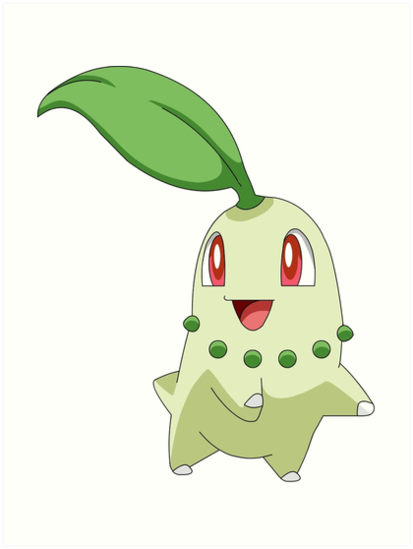
\includegraphics[scale=0.5]{gfx/chikorita.png}
%\caption{Aqui esta chikorita}
%\end{figure}

La mecánica estadística y la economía son consideradas como dos campos de investigación diferentes, el primero que pertenece a la rama de la física y ciencias naturales, y la segunda a las ciencias sociales.
Sin embargo, a partir del siglo XIX la evolución en la investigación de la economía permitió establecer analogías entre las dos ciencias.
De este modo la economía puede ser estudiada desde el punto de vista de la física estadística.

En este capitulo se presenta al lector los conceptos esenciales para comprender las analogías Física-Economía aplicadas en esta Tesis.
Se introducirán ciertos conceptos clave de Economía para la compresión de esta Tesis.
Del mismo modo, vamos a presentar los conceptos de mecánica estadística que son aplicados. 
En este Capítulo se introducirá al lector al estado del arte de la econofísica y sobre todo, la aplicación del concepto de entropía a la economía.
Finalmente, se presentarán aplicaciones de la econofísica a las finanzas y mercados actuales.

\section{La similitud entre economía y física}


En \textit{Física}, un sistema cerrado conserva la energía,  en \textit{Economía}, un sistema económico cerrado conserva el \textit{dinero}. 
De la anterior analogía se entiende que no hay un flujo externo de dinero, por lo que la cantidad total de dinero se conserva.

La \textit{mecánica estadísitica} estudiada por los físicos, y la economía, tienen en común que ambas estudian grandes ensambles; colecciones de átomos, y agentes económicos, respectivamente.
\citep[][pagina 149]{cottrell_classical_2009}.

\textit{De la anterior analogía, en una colección de átomos se asume que cada uno de ellos posee una energía cinética $\mathit{\varepsilon}_{i} \geqslant 0 $, mientras que en los mercados financieros cada uno de los agentes participantes tiene un recurso llamado dinero el cual no puede ser negativo, es decir  $\mathit{d}_{i} \geqslant 0 $} \citep[][pagina 149]{cottrell_classical_2009}.




Adicionalmente, en \textit{Física}, a menudo se dice que un sistema se encuentra en equilibrio cuando la energía con que interactúan los componentes es conservada. 


\subsection{Economía neoclásica} 

En los comienzos de la \textit{Econofísica} se encuentran emblemáticos personajes como Adolphe Quétlet(1796-1874), Léon Walras (1834-1910), Vilfredo Pareto (1848-1923), y Adam Smith (1723-1790), quienes ofrecieron un conjunto de ideas que permitieron ampliar la manera en que se estudia la \textit{Economía}.
Una de sus mayores contribuciones es considerar una transacción como una consecuencia determinista del intercambio de bienes entre dos agentes.
Esta consideración es innovante con respecto al las corrientes económicas y sociales del siglo XIX (e.g. aspectos sociales,  factores políticos, distribución de la riqueza). 

Esta inovación permite a la \textit{Econofísica} estudiar los sistemas complejos intrínsecos de la \textit{Economía}. La \textit{Econofísica} entonces considera que un sistema complejo esta compuesto de un gran número de \textit{grados de libertad} en diferentes escalas de tiempo  \citep[][pagina 17]{richmond}.

La \textit{Economía neoclásica} puede ser considerada como la corriente de pensamiento que da lugar a la \textit{Econofísica}. Del mismo modo que Pareto estudió la distribución de la riqueza en el siglo XIX, Adam Smith propuso la descripción de un fenómeno llamado \textit{la mano invisible}. 
Este y otros conceptos de economía pueden ser consultados en el capítulo \ref{glosario}.

\subsubsection*{Función de utilidad}

Se utiliza para encontrar el numero óptimo de diferentes profesionales en una compañía, también se utiliza para hallar la mejor elección de acciones de un mercado \citep[][]{richmond}. 


\subsection{Retornos} 
%---------------------------------------------------------------------------
%Introducir RETORNOS en el texto
%Se define como  r($\mathit{t_{i}}$) $\equiv $ \textit{x}$(\mathit{t}_{i})$ - \textit{x}($\mathit{t}_{i} - \Delta t$) , donde \textit{x}($\mathit{t}_{i}$ es una secuencia de precios logarítmicos 
Los retornos son usualmente variables de análisis más rentables que el precio perse, por varias razones. 
La distribución de los retornos es más simétrica y estable en el tiempo que la distribución de los precios en sí. 
La estructura de los retornos es cercana a estacionaria, mientras que la estructura de los precios observados en el tiempo no lo es \citep[][pagina 17]{dacoragna}.

El logaritmo de los precios muestra que están normalmente distribuídos, al menos aproximadamente \citep[][]{osborne}. En esta Tesis se trabaja con los retornos de los registros diarios individuales de cada serie de tiempo financiera, en otras palabras, la ventana temporal entre cada \guillemotleft tick\guillemotright~ es constante y entonces el \textit{lag} que se se denota como $\delta t$ poseé el valor constante de un día. 


Los retornos son expresados como:
\begin{center}
$R_t=P_{t+1}-P_t$~~.
\end{center}
Es decir, el retorno del precio en cuestión ( $R_t$ ) es equivalente al precio individual de su sucesor temporal ( $P_{t+1}$ ) menos el precio del objeto temporal en turno ( $P_t$ ), sin embargo, siguiendo los ideales de Osborne, hay que calcular el logaritmo de los retornos a sabiendas de que los precios se etiquetan como $\mathit{Z_t}$ y son las variables de registro de las mediciones individuales diarias al cierre del mercado, donde \newline $t \in \mathcal{T} = \{\mathit{T_1,T_2,\ldots , T_M}\}$. El logaritmo del precio es:

\begin{center}
$\mathit{Y_{t}} = $ ln $\mathit{Z_{t}}$~~.
\end{center}

Entonces los \textit{retornos logarítmicos} son definidos como: 

\begin{center}
$X_t = $ $\mathit{Y_{t}} - $  $\mathit{Y_{t - 1}}$~~.
\end{center}

Cuya interpretación es la diferencia sucesiva de los logaritmos de los precios  registrados en el tiempo, en otras palabras, la diferencia del logaritmo del precio en turno y su antecesor temporal. Aunque en términos computacionales es mucho más sencillo trabajar con la siguiente expresión que respeta la proposición de Osborne\citep[][]{slanina}: 
\begin{center}
ln $R_t = $ ln $\mathit{P_{t+1}} - $ ln $\mathit{P_{t}}$.
\end{center}%esto fue sacado de la pagina 132 y 133 del libro essentials of econophysics modeling


\subsection{Propiedades de los retornos}
\label{retornos}
Podemos citar algunas propiedades de los retornos propuestas por \cite{Cont2001}:

\begin{itemize}
	\item {Ausencia de auto correlación: Las autocorrelaciones lineales no son significativas en la mayoria de los casos}
	\item {Colas largas: La distribución de retornos parece seguir una ley de potencias.}
		%the (unconditional) distribution of returns
		%seems to display a power-law or Pareto-like tail, with
		%a tail index which is finite, higher than two and less
		%than five for most data sets studied. }
	\item Asimetría Ganancia/Perdida: Se observan bajas más claramente que altas en los precios. 
	\item Gaussianidad agregada (aggregational gaussianity): cuando se aumenta el intervalo de tiempo en el que se calculan los retornos se observa que el valor de los retornos sigue una distribución gaussiana. 
	\item Intermitencia: los retornos muestran un gran grado de variabilidad.
	\item Asimetría en escalas de tiempo: a mayor intervalo de tiempo los retornos muestran volatilidad más fácilmente que cuando el intervalo de tiempo es menor.
\end{itemize}

Además de las propiedades listadas arriba, algunas definiciones de mercado eficiente implican que los retornos no son predecibles. Por ejemplo, Arthur Stalla-Bourdillon de la Banca de Francia en su articulo \textit{Stock Return Predictability: comparing Macro- and Micro-Approaches} \citep{stalla-bourdillon_stock_2022} da el siguiente ejemplo:
\begin{quotation}
\textit{Dado que toda la información está contenida en los precios del mercado, los cambios en el mercado pueden solo ser causados por la llegada de nueva información, que es por definición, es impredecible. En otras palabras, los precios deben seguir una caminata aleatoria; una regresión de retornos basada en información pasada no debe contener información predictiva}.
\end{quotation}
La predictividad de los retornos así como sus propiedades estadísticas son discutidas en profundidad por \cite{Pesaran2010}.
En su artículo, Pesaran menciona que la predictibilidad de los retornos puede ser asociada a la volatilidad del mercado sugiriendo que la predictividad se incrementa en tiempos de crisis. 

A continuación se describen las propiedades anteriormente mencionadas con la finalidad de que sean aterrizadas en el contexto de esta Tesis.

La ausencia de auto correlación como indica la primera propiedad se refiere a que los registros de los precios de cada día no producen un objeto de análisis en la mayoría de los casos, aunque dichos registros sean parecidos entre sí.

La tercera propiedad propuesta por \cite{Cont2001} se refiere a que los retornos  permiten identificar aquellos registros en que hubo pérdida en vez de ganancia, en cuyo caso sería un valor negativo para el retorno.

El cuarto punto hace referencia a que si se consideran todos los registros de un mercado los retornos asemejarían una distribución gaussiana.

Con respecto a la quinta propiedad. Los retornos fluctúan entorno a una media pero ello no implica que el valor de los retornos se comporte constante o que muestre una tendencia.

La sexta propiedad propuesta significa entre mayor sea el período de tiempo que conforma a una colección de retornos, menor será la simetría y mayor la volatilidad entre ellos.

\section{Analogías Física-Economía} 
\subsection{Ley de Boltzmann-Gibbs y distribución de la probabilidad del dinero (en equilibrio)} 

La \textit{ley de la distribución de la probabilidad de la energía} en la \textit{mecánica estadística}:

\begin{center}
$\mathit{P(\varepsilon)} = $ C $e^{-\varepsilon/\mathit{T}}$,
\end{center}
donde:

$\varepsilon$ es la energía

$C$ es una constante de normalización

$\mathit{T}$ es la temperatura (Wannier,1966) 

Dada la similitud de un sistema descrito por la Ley de Boltzmann-Gibbs y las condiciones de un sistema económico cerrado, por analogía se tiene que esta ley es una descripción de la \textit{distribución de la probabilidad del dinero}
\citep[][]{cottrell_classical_2009}.


\subsubsection{Distribución de la probabilidad del dinero (en equilibrio)}


De acuerdo con Cottrel, Michelson y Wright \citep[][]{cottrell_classical_2009} la distribución de la probabilidad del dinero sigue la forma de la \textit{Ley de Boltzmann-Gibbs}


\begin{center}
$\mathit{P(d)} = $ C $e^{-d/\mathit{T}}$,
\end{center}
Donde:

$d$ es el dinero

$C$ es una constante de normalización

$\mathit{T}$ es el promedio de la cantidad de dinero por agente en el sistema económico.

Con base en el artículo \textit{Price variations in a stock market with many agents} por Shubik, Pakzuski y Bak en 1997, la ley de la conservación del dinero establece que el dinero no puede ser manufacturado por agentes del sistema económico pero si puede ser transferido entre ellos. Esta descripción es análoga a la que un sistema conservativo presenta en Física, por ejemplo, cuando en un sistema cerrado sin intercambio de energía con el exterior, los átomos colisionan entre sí \citep[][]{shubik}. 
\newpage

\subsubsection{Ley de la conservación del dinero.} 

En relación con lo establecido por Shubik, Pakzuski y Bak en 1997 en el artículo ya mencionado, lo que compete en este trabajo de Tesis es el resultado de la interacción entre los agentes \textit{i} y \textit{j}. 

Sean \textit{i} y \textit{j} dos agentes que interactúan en el mercado, correspondiéndole a cada uno de ellos una cantidad finita de dinero $d_{i}$ y $d_{j}$ respectivamente, se puede denotar de la siguiente manera: $[d_{i},d_{j}]$. 

Si al llevarse a cabo la interacción entre dos agentes y el intercambio de dinero que llevan a cabo es constante, dicho intercambio se etiqueta como $\Delta d$. El resultado de la interacción de los agentes en cuestión se expresa como:  $[d_{i},d_{j}]$ $\longrightarrow$  $[d'_{i},d'_{j}] = [d_{i} - \Delta d ,d_{j} + \Delta d]$. Dicho lo anterior puede notarse que $d_{i} + d_{j} = d'_{i} + d'_{j}$ lo cual significa que la cantidad total de dinero en la transacción es conservada si no existe un flujo externo de dinero que modifique la cantidad total $d$.

En tales condiciones se asume que la distribución de probabilidad del dinero en equilibrio es invariante pese a fuertes fluctuaciones $\Delta d$ entre los agentes \citep[][pagina 149]{cottrell_classical_2009}.


%Ahora que se ha comprendido que el intercambio de dinero $\Delta d$ entre %los agentes es la interacción elemental para la existencia de la %\textit{Economía}, es momento de entender el funcionamiento de la %\textit{Economía neoclásica} para poder utilizar el concepto de %\textit{caminata aleatoria} mismo que se utiliza para sentar las bases del %concepto de \textit{mercado eficiente}.

como descrito en \citep{Huang2021}.



\subsection{Segunda Ley de la termodinámica y la Segunda Ley de la econofísica} 


%
%Este concepto ha sido discutido por \cite{hernandez-montoya_entropy_2022}.
%El concepto de entropia ha sido largamente estudiado \citep{hernandez-montoya_entropy_2022}.

%El concepto de entropia ha sido largamente estudiado \citep[ver mas informacion en ][]{hernandez-montoya_entropy_2022}.


%Para mas infor ver \citep{hernandez-montoya_entropy_2022,jakimowicz_role_2020,martinez_alisis_nodate}.
Existe una formulación conocida por Kelvin-Planck que dice : \textit{No hay proceso termodinámico en estado constante para el cual el calor es completamente convertido en trabajo} \citep[][pagina 86]{struchtrup}.

Sin embargo, la primera derivación de la segunda ley fué dada por Rudolf Clausius (1822-1888) basada en el argumento de que la dirección en que se transfiere el calor esta restringida y depende estrictamente de las declaraciones en ciclos termodinámicos \citep[][pagina 55]{struchtrup}.  Del desarrollo de la segunda ley por Clausius se tiene que \textit{el calor irá del calor al frío por sí mismo, y no al revés} \citep[][pagina 64]{struchtrup}.

La segunda ley explica la restricción en la eficiencia y la dirección de los procesos, \textit{el calor no puede ser completamente convertido en trabajo} \citep[][pagina 5]{struchtrup}. 

Lo anterior se ha definido en la literatura mediante la siguiente ecuacuón:

\begin{equation}
dS \geqslant \frac{\delta Q}{T},
\end{equation}

donde $\delta$ es la diferencial inexacta del calor $Q [J]$ , entre la temperatura $T [K]$, mientras que $dS$ es el diferencial de la entropía $S$ $\frac{[J]}{[K]}$. Esta relación indica que la entropía es incrementada en procesos espontáneos pero no cambia en equilibrio \citep[][pagina 340]{keszei2011chemical}. 

\subsubsection{Segunda Ley de la econofísica} 

Por analogía con la sección anterior, se llama a $S$ como $S_e$ que es la entropía económica (Georgescu-Roegen, 1971), aunque $S_e$ será una cantidad adimensional, mientras que la constante $\lambda$ es un factor integrante cuya unidad de medida es la moneda según sea el caso \citep[][pagina 166]{richmond} , y en vez de $Q$ se ocupa $M$ que en este caso es el dinero. 

\begin{equation}
dS_e \geqslant \frac{\delta M}{\lambda}
\end{equation}

Es preciso mencionar que en Economía $S_e$ se le llama función de producción. En el presente trabajo de Tesis no se determina el factor integrante, aunque existen métodos para obtenerlo. Aunque no es precisamente análogo dicho factor integrante a la temperatura, vale la pena mencionar que desde el punto de vista de la Física, en termodinámica se utiliza la constante de Boltzmann como enlace entre temperatura y energía \citep[][pagina 166]{richmond}. 

Para terminar de comprender la relación de las variables entre la segunda ley de la termodinámica y la segunda ley de la econofísica se presenta la siguiente Tabla. 

\begin{table}	
	\begin{center}
		\begin{tabular}{ |l |r | l | c| }
			\hline
			Economía &  Unidades & Física & Unidades  \\ \hline
			M dinero & moneda & Q calor & joules $[J]$ \\
			K capital & moneda  & E energía & joules $[J]$\\ 
			P producción &  moneda   & W trabajo & joules $[J]$ \\
			$\lambda$ fluctuación & moneda & T temperatura & kelvin $[K]$\\ 
			$S_e$ entropía económica & adimensional & S entropía física & $\frac{J}{K}$ \\
			$\pi$ presión económica & moneda circulante & P presión & $\frac{N}{[m]^{2}}$\\
			A libertad de acción & adimensional & V volumen & $[m]^{3}$ \\
			\hline
		\end{tabular}
		\label{tab_analogiasFisEcono}
		\caption{Variables importantes en sistemas económicos y físicos.}
	\end{center}
\end{table}

\subsection{Entropía en la termodinámica y analogía en la econof\'isica} 

Para Clausius en 1865 la entropía es una energía inutilizable que puede provenir de por ejemplo, de un motor de vapor que utiliza combustible, irremediablemente una cantidad de energía no será aprovechada. Adicionalmente sostiene que la energía inutilizable en el universo o cualquier sistema cerrado tiende a incrementar \citep[][pagina 21]{cottrell_classical_2009}. 

La entropía es una cantidad que surge cuando se construye una desigualdad que describe la tendencia al equilibrio  \citep[][pagina 70]{keszei2011chemical}. 

%\subsection{Entropía en la econofísica} 

En el contexto de econofísica, la entropía es la medida de un número total de microestados económicos accesibles o disponibles que pertenecen a un macroestado ( mercado-estado fase "económico"). Aqui la analogía se encuentra en que, la energía mide la probabilidad para que un estado en particular en un espacio fase "económico" sea alcanzado. (pg.200, Richmond, Econophysics) \citep{cottrell_classical_2009}.

\subsection{Entropía en la mecánica estadística} 


Es la medida de un número total de microestados económicos accesibles o disponibles que pertenecen a un macroestado ( mercado-estado fase "económico"), por analogía, la energía mide la probabilidad de que un estado en particular en un espacio fase "económico" sea alcanzado \citep{richmond}.

\subsection{La ecuación de la entropía}

La ecuación de Boltzman para la entropía está definida como:

\begin{equation}
	S = -k_B \int p(\Gamma,t) ln p(\Gamma,t) d\Gamma.
	\label{entropyB}
\end{equation}
En esta ecuación la entropía $S$ es definida para moléculas en un espacio fase determinado  en un macroestado termodinámico.
En la ecuación \ref{entropyB} $k_B$ es la constante de Boltzmann, $ p(\Gamma,t)$ es la función de densidad de probabilidad en el tiempo de $\Gamma$. $\Gamma$ engloba a las variables de posición y momento del espacio fase \citep[][pagina 13]{richmond}. Cabe mencionar que un macroestado esta relacionado con las variables temperatura, presión y volumen.
 
Por otro lado, en el estudio de microestados discretos contables y accesibles, la ecuación de la entropía es: 
 
 \begin{equation}
 	S = -k_B \Sigma p_r ln p_r.
 \end{equation}  

Donde $p_r$ es la probabilidad de un microestado. 

Otra definición de la entropía es dada por la ecuación de Shannon \ref{entropySha}.
En este trabajo de Tesis se define como la cantidad de pérdida y ganancia de información en un conjunto de datos.

\begin{equation}
	H = - \sum_{n=1}^{n} p_i log(p_i).
	\label{entropySha}
\end{equation}

Donde $p_i$ es la probabilidad del dato en cuestión. 

\section{Aplicaciones de la ecuación de Shannon para la entropía.}

Aunque este trabajo de Tesis no está orientado a la inteligencia artificial (AI por sus siglas en inglés), resulta interesante que la AI aplica el concepto de entropía de la información. 
Por ejemplo en el portal tds (towards data science) \citep[][]{tds} en la publicación \textit{Entropy and Information Gain in Decision Trees} se utiliza el concepto de entropía para analizar la impureza de una base de datos. 
Su interés ha sido analizar las edades de las personas y los alimentos de su preferencia. 
Su método aplica una reducción en la entropía antes de procesar la base de datos con un árbol de decisiones. 
Esto permitió tener una ganancia de información\citep[][]{tds}, y de dicha ganancia de información se obtiene si la persona que entrevistan respecto a sus preferencias por diferentes alimentos es o no es del medio oeste de los Estados Unidos. Su objetivo era mostrar que mediante la aplicación del método de la ganancia de entropía a los árboles de decisiones se puede llegar a la homogeneidad de los datos, en cuyo caso la entropía sería cero

En este punto resulta interesante comprender el alcance que tiene la ecuacion de Shannon, no solamente en la termodinámica. 
Otro ejemplo es presentado en la publicación \textit{Entropy Calculation, Information Gain and Decision Tree Learning} del sitio web medium \citep[][]{medium} , donde se utiliza el concepto de la homogeneidad y no homogeneidad de la información para mejorar el modelo de árboles de decisiones. Se 
menciona que la impureza de la información será cero si todos los registros son de una misma clase, y si se dividiera en dos clases y hay exactamente la misma cantidad de registros para cada una de las clases, entonces se tendría una impureza del 100 porciento o una colección completamente no homogénea de registros. 
En inteligencia artificial un árbol de decisiones es frecuentemente utilizado como clasificador de bases de datos.
Calcular la entropía permite tomar los atributos más importantes de la base de datos para conformar un árbol de decisiones, así como medir la homogeneidad de los datos. 
Por consecuencia, puede ayudar a determinar la calidad del árbol de decisiones. 

En otra publicación \citep{dos2012entropy}  , se utiliza el mismo concepto de un árbol de decisiones. 
En este caso se tiene como objetivo que el algoritmo de inteligencia artificial determine el impacto de un atributo con respecto otro basado en la cantidad de información que presentan para así clasificar tareas. 

La ecuación de la entropía de Shannon no solamente se aplica para árboles de decisión, también se ha utilizado para mostrar que algunos textos poseen más riqueza en su contenido con respecto a un tema. 
Además se menciona que en comparación con las técnicas tradicionales del aprendizaje-máquina la aplicación de la entropía de Shannon disminuye la tasa de falsos positivos en relación con las palabras clave que se refieren a un tema en particular \citep[][]{chan2022knowledge}.   
 
\subsection{La entropía aplicada a la econofísica}

Una primera aproximación es considerar la entropía como un cálculo de estructuras complejas. Las estructuras con entropía alta tienen poca información que aportar, y las estructuras con baja entropía pueden ser consideradas determinísticas \citep[][]{pincus2004irregularity}.

Un \textit{mercado eficiente} es una estructura con máxima entropía, y entre más alta es la entropía del mercado más eficiente es el mercado.

Una segunda aproximación esta dada a partir de la definición de Boltzmann, su aplicación en el contexto de econófisica es la medida del número total de estados económicos accesibles \citep[][]{richmond}. Es decir, la oportunidad temporal que poseen los agentes para interactuar en el mercado.

Una tercera manera es la que se emplea en macroeconomía. La función de utilidad es conocida como función de producción $S_e$, en referencia a que se ha etiquetado a $S$ como la entropía. 

La primera y segunda leyes de la econofísica se aplican directamente en este contexto, ya que la entropía captura información crucial. Por ejemplo, la función de producción $S_e$ se obtiene de la cantidad de personas contratadas en diferentes ocupaciones y cuantas unidades producen \citep[][pagina 170]{richmond}. 

Una cuarta manera de acercarse a este concepto de la manera en que se aborda en esta Tesis es a través del uso que se le da la entropía como función de utilidad en econofísica. El concepto de función de utilidad se ha definido en la Economía neoclásica. Entonces en el contexto de la Economía neoclásica la entropía se obtiene considerando el número total de elementos que pertenecen a la colección número uno, el número total de elementos pertenecientes a la colección número dos, y así sucesivamente. 


Dentro de esta misma aproximación y en el contexto matemático, se interpreta a la maximización de la función de producción lo que implica estudiar la entropía a través de un Lagrangiano \citep[][página 205]{richmond} \citep[][página 150]{cottrell_classical_2009}.

De igual manera, un acercamiento a este concepto en la vida cotidiana se encuentra en la maximización  de la entropía, o bien, la maximización de la función de utilidad es el numero óptimo de empleados para desarrollar una óptima producción.

De este cuarto punto de vista se concluye que la entropía vista desde la Economía es una función de producción. 

Una quinta aplicación de la entropía en la econofísica es en el estudio del precio específico que se denota como $\psi$, el cual es el valor por hora del contenido laboral \citep[][]{cottrell_classical_2009}. La distribución de $\psi$ permite que se pueda calcular la ecuación entropía de Shannon. De lo anterior se encuentra que con una desviación estándar pequeña hay una baja entropía, y cuando la desviación estándar es grande se tiene una entropía grande \citep[][pagina 189]{cottrell_classical_2009} (ver Figura \ref{entropia-cottrel)}.

\begin{figure}
	\centering
	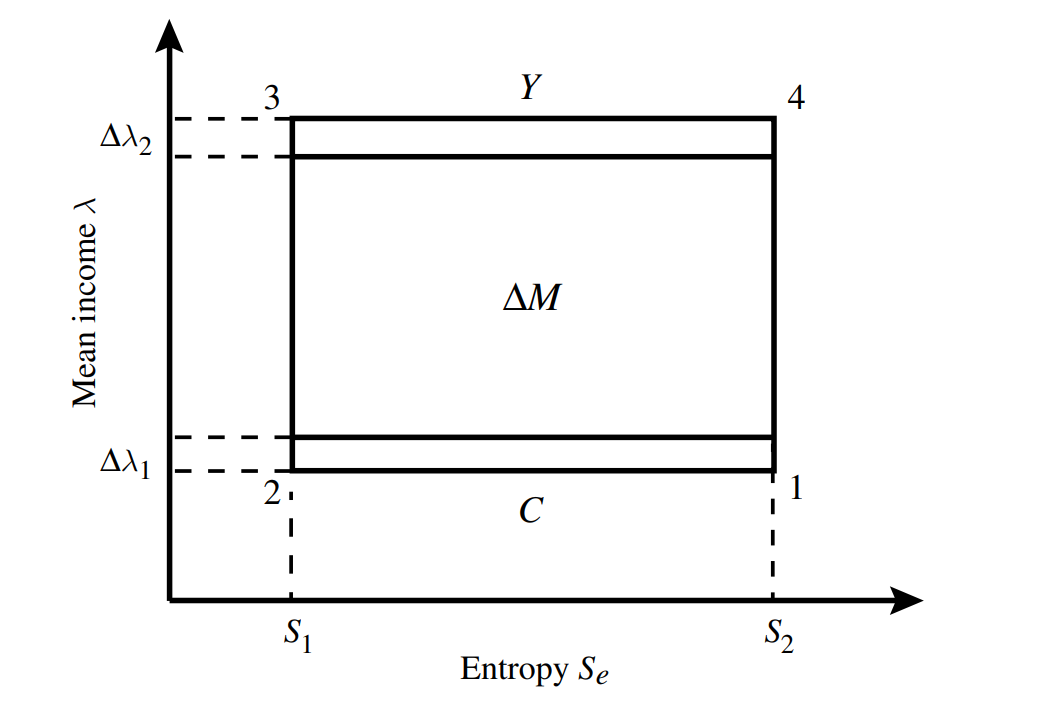
\includegraphics[width=0.7\linewidth]{figures/image_2023_05_02T13_03_47_409Z}
	\caption{Representación de como una desviación estándar pequeña tiene una baja entropía, y viceversa, una gran desviación estándar posee una entropía muy alta.}
	\label{entropia-cottrel}
\end{figure}


Adicionalmente, Richmond muestra una serie de ejemplos en los que la entropía se estudia en situaciones estrechamente aplicadas a la economía. En su explicación muestra una analogía con el ciclo de Carnot (ver Figura \ref{entropia-Richmond}. 

\begin{figure}
	\centering
	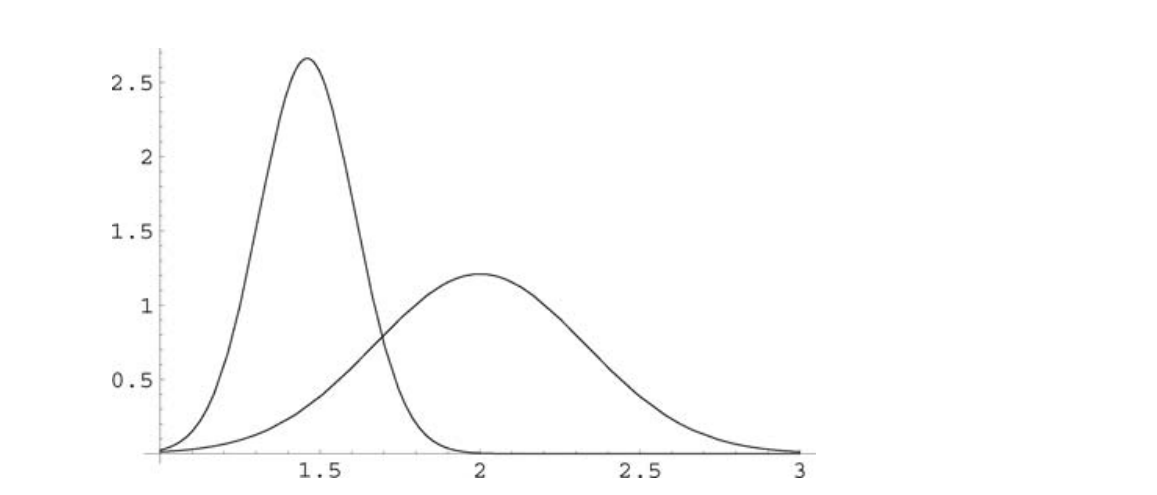
\includegraphics[width=0.7\linewidth]{figures/image_2023_05_02T13_19_46_895Z}
	\caption{Mecanismo de crecimiento económico. El excedente $\Delta M	~=~\Delta M_1~+~\Delta M_2$ con 
	$\Delta M_1~=~\Delta \lambda_1\Delta S_e$ y $\Delta M_2~=~\Delta \lambda_2\Delta S_e$ (aquí $\Delta \lambda_1$ es el dinero con el que se compra y $\Delta \lambda_2$ es el dinero de venta) dan pie a la continuación del ciclo de Carnot en los niveles $(\lambda_1~=~ \Delta\lambda_1)$ y $(\lambda_2~=~ \Delta\lambda_2)$.}
	\label{entropia-Richmond}
\end{figure}


En el diagrama $C$ se refiere al costo, $\Delta M$ significa la ganancia en el proceso de producción,  \textit{Y} significa los ingresos, $\lambda$ es el estándar de vida, aunque es más apropiado interpretarlo como el \textbf{dinero} que posee un agente en un punto en particular, donde $\lambda_{1}$ es dinero con que se compra mientras que $\lambda_{2}$ es el dinero de venta, y $S_e$ es la entropía desde el punto de vista de la economía por lo que también se le puede denominar como función de producción.

Entonces una sexta aplicación de la entropía es el de los granjeros en el mercado tal como se muestra en la siguiente Tabla (ver Tabla \ref{tab_manzanas}). Cabe mencionar que la flecha $\rightarrow
$ indica \textit{se convierte en}.  

De la misma manera Richmond explica que la entropía también se puede estudiar en ciclos monetarios. Así una séptima manera de estudiar la entropía es la descrita en la Tabla (ver Tabla \ref{tab_dineroManzana} ). 

\begin{table}	
\hskip-4.0cm\begin{tabular}{ |l |r | l | c| }
		\hline
		Punto en el ciclo &  Acción & Entropía & Dinero  \\ \hline
		1 $\rightarrow$ 2 & Manzanas recolectadas en una plantación  & $\Delta S_{e} < 0 $ &  $\lambda_{1}$ \\
		 &  al costo más bajo & &   \\ \hline
		2 $\rightarrow$ 3 & Manzanas traídas de la plantación & $\Delta S_{e} = 0 $ & $\lambda_{1} \rightarrow \lambda_{2}$\\ 
		 &  al mercado  &  & \\ \hline
		3 $\rightarrow$ 4 &  Manzanas distribuídas a consumidores   &$\Delta S_{e} > 0 $ & $\lambda_{2}$ \\  
		&  a alto precio   & & \\  \hline
		4 $\rightarrow$ 1 & Fertilizantes a partir de residuos &  $\Delta S_{e} = 0 $  &  $\lambda_{2} \rightarrow \lambda_{1}$\\  
		 &  son llevados al campo &   &  \\  
		\hline
	\end{tabular}
	\label{tab_manzanas}
	\caption{Manzanas producidas en una granja a precio $\lambda_{1}$ y vendidas al mercados en $\lambda_{2}$. }
\end{table}


\begin{table}	
	\hskip-4.0cm\begin{tabular}{ |l |r | l | c| }
		\hline
		Punto en el ciclo &  Acción & Entropía & Dinero  \\ \hline
		4 $\rightarrow$ 3 & Agricultor obtiene dinero de clientes & $\Delta S_{e} < 0 $ &  $\lambda_{2}$ \\
		& que compran a precio alto & & \\ \hline
		3 $\rightarrow$ 2 & Manzanas traídas de la plantación   & $\Delta S_{e} = 0 $ & $\lambda_{1} \rightarrow \lambda_{2}$\\ 
		& al mercado  &  & \\ \hline
		3 $\rightarrow$ 4 &  Manzanas distribuidas a consumidores  &$\Delta S_{e} > 0 $ & $\lambda_{2}$ \\
		& a alto precio   & &  \\  \hline
		4 $\rightarrow$ 1 & Fertilizantes a partir de residuos &  $\Delta S_{e} = 0 $  &  $\lambda_{2} \rightarrow \lambda_{1}$\\  
		&  son llevados al campo &  &  \\  
		\hline
	\end{tabular}
	\label{tab_dineroManzana}
	\caption{Manzanas producidas en una granja a precio $\lambda_{1}$ y vendidas al mercados en $\lambda_{2}$. }
\end{table} % contexto teorico
% !TEX root = ../thesis-example.tex
%
\chapter{Metodologia}
\label{Metodologia}

Descripcion de metodo aplicado para entropia  ver diagrama \ref{diagramaentropia1}.

Para comenzar, los datos se han obtenido a través del portal Yahoo Finance, por lo que son registros del precio de cierre de cada dia, además dichos datos fueron depurados y ordenados ya que había algunos espacios en blanco en el archivo original, entonces el software con que se trabaja interpreta los datos sin errores. 

Luego que se han cargado los datos, y se han ordenado es necesario calcular los retornos de los precios. La razón por la que se trabajan los retornos de los precios y no se trabaja directamente con los precios ya que no poseen estacionaridad en el tiempo y ello conlleva a que no va a haber una media central en los datos. Los retornos permiten que los datos se encuentren entorno a una media.

Aunque los retornos son una mejor representación de los precios, aún presentan picos que sobresalen de la media, por lo que se estandarizan los retornos, la estandarización permitirá destacar aquellos retornos que realmente poseen picos en su valor de retorno. 

Ya que cada retorno ha sido estandarizado con su respectiva fecha,  se procede a discretizar los retornos mediante un proceso que divide en cuatro intervalos a los retornos. Determinar los cuartiles de los retornos y discretizarlos con base en la etiqueta que se pone a cada intervalo, en otras palabras, los intervalos van a permitir etiquetar del 1 al 4 a cada retorno. 

La ecuación de la entropía requiere conocer la probabilidad de los elementos del sistema, con los intervalos dados por los cuartiles y la discretización de los retornos se obtiene todo lo necesario para calcular la entropía, sin embargo, no se calcula la entropía de todo el conjunto de datos, se hace por subconjuntos de datos agrupados en listas de 50 elementos, o cualquier número dado por el usuario.

El resultado de la entropia es dado en valores y fechas para cada subconjunto de días.

\begin{figure}
	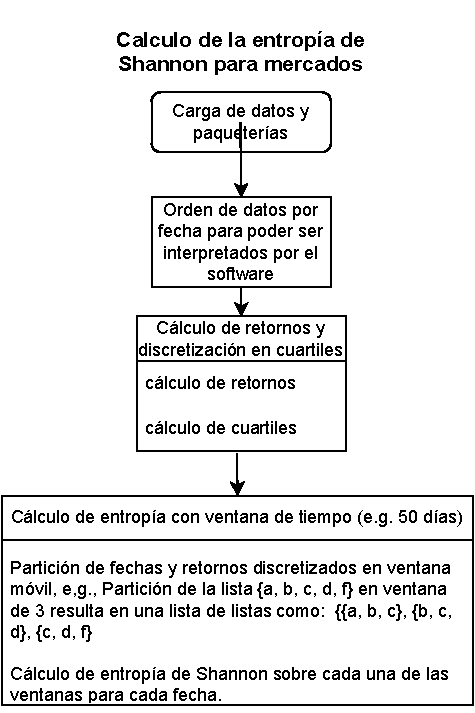
\includegraphics[width=0.7\linewidth]{figures/diagrama_entropia1}
	\caption{Diagrama del algoritmo utilizado para el c\'alculo de entrop\'ia de Shanon en mercados financieros.}
	\label{diagramaentropia1}
\end{figure}


Descripcion de metodo aplicado para entropia utlizando medias moviles ver Figura \ref{entropiamav} . 
Se aplica el mismo metodo mencionado arriba, adicionalmente en la etapa en que se estandarizan los retornos de los precios con su respectiva fecha. La ventana puede ser elegida por el usuario. Se aplica una entrada de por lo menos 50 días ya que un número menor no suavizaría la curva de manera que no se podría apreciar tendencias en el comportamiento de la curva.





\begin{figure}
	\centering
	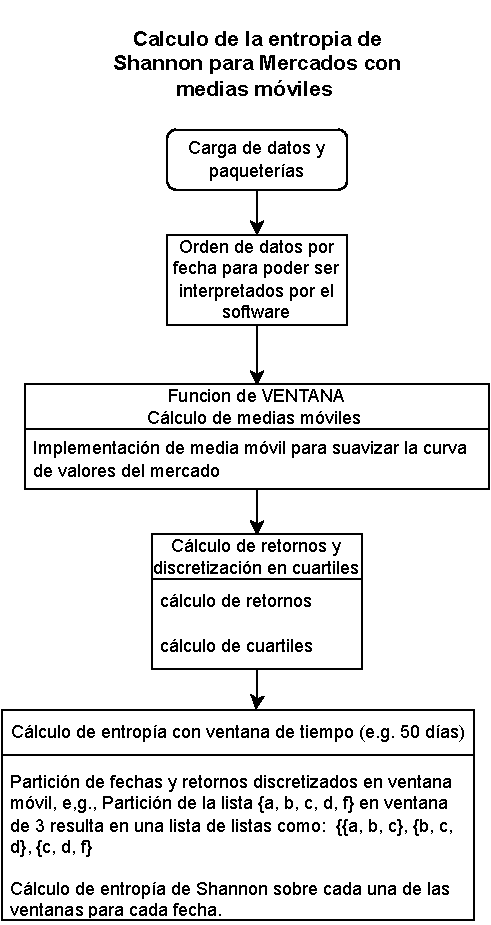
\includegraphics[width=0.7\linewidth]{figures/entropiaMAV}
	\caption{Diagrama del algoritmo utilizado para el c\'alculo de entrop\'ia de Shanon en mercados financieros con medias m\'oviles.}
	\label{entropiamav}
\end{figure}

La simulación de un mercado eficiente requiere cargar datos debido a que se simula un caminante aleatorio a partir de una distribución gaussiana con una media y desviación estándar obtenidas del análisis de los retornos (no estandarizados) de los precios reales. 

Del paso anterior se obtienen retornos simulados, mismos que deben estandarizarse y asignarles su fecha.

A partir de este punto hay dos situaciones que se pueden apreciar en el diagrama \ref{simulacion}, la primera es que a dichos retornos simulados se les aplica el proceso para el cálculo de entropía de la figura \ref{diagramaentropia1}, y la segunda es que se aplica el proceso de medias móviles como se presenta en \ref{entropiamav}.


Se destacan valores mínimos de entropía gracias a la manera en que se presentan los resultados, con ello comparar el comportamiento de la entropía del mercado eficiente y del mercado real con fechas, con o sin media móvil requiere únicamente del cálculo de un umbral que diferencie los valores de entropía que se comportan de manera gaussiana  de los que no.

Mediante la definición de un umbral que permite seleccionar con un intervalo de confianza de 95 porciento los valores de entropía mínima en los mercados. 

\begin{figure}
	\centering
	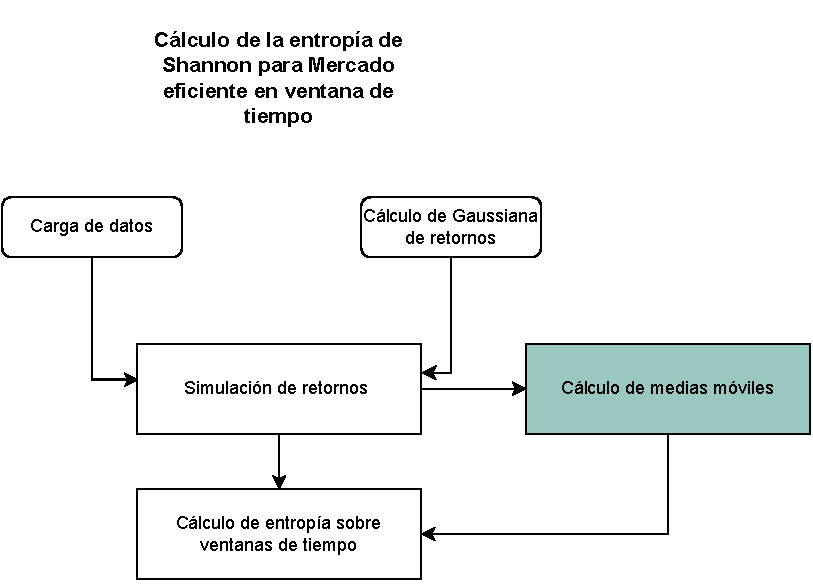
\includegraphics[width=0.9\linewidth]{figures/simulacion}
	\caption{Diagrama del algoritmo de calculo de entropia para la simulacion de mercado eficiente. }
	\label{simulacion}
\end{figure}

Reglas de cuartiles
\begin{center}
	\begin{tabular}{ |r | l | c| }
		 \hline
		Cuartil & Regla & etiqueta \\
		primer cuartil & $\inf > 0$ & 1 \\
		2 &   & Calculo de madia moviles utilizando N dias\\ 
		3 &     &Estimacion gaussiana con sigma igual 3 \\
		 \hline
	\end{tabular}
\end{center}



Finalmente, se aplica una prueba estadística de distribuciones a los valores con mínima entropía, tanto de aquellos que fueron tratados con un filtro de media movil como aquellos que no. 	% INCLUDE: system
% !TEX root = ../thesis-example.tex
%
\chapter{Conceptos}
\label{sec:related}

\cleanchapterquote{Un sistema físico macroscópico no puede ser descrito solo en términos de variables mecánicas, la llamada entropía era necesaria}{P. Richmond, J. Mimkes, S. Hutzler}{(2013)}




{
    \noindent
 Los conceptos que se presentan a continuación son manifestados en el orden en que se tenga el mayor entendimiento de este trabajo de tesis, no debe confundirse la nomenclatura, ya que 1. se ocupa para todo aquello relacionado directamente con \textit{econofísica} y 2. se ocupa para todo aquello relacionado con \textit{Economía}.\newline
}

{
\noindent
\Large \textbf{1.1.1. Econofísica}
}

Término acuñado por Eugene Stanley en 1997 para referirse a una rama de la Física\citep[][página 3]{roehner2002patterns} que a partir de encontrar relaciones entre leyes físicas y variables macroscópicas propias de la Economía, busca un entendimiento más profundo de los fenómenos que en esta se presentan en los mercados. 
\newline

{
\noindent
\Large  \textbf{2.1.1. Economía} 
}

Es el estudio de cómo las sociedades utilizan recursos escasos para producir bienes valiosos y distribuirlos entre diferentes personas \citep[][]{samuelson2009economics}.
\newline

{
\noindent
\Large  \textbf{1.2. Agentes} 
}

Son los individuos, compañías, países, casas de bolsa, familias, comercientes, inversionistas, capaces de interactuar entre sí de una manera no trivial, que además se encuentran inmersos en un mecanismo auto-organizado pese a poseer intereses particulares cada uno.
\newpage

{
\noindent
\Large  \textbf{1.3. Modelo de agentes} 
}

Estructuras presentes en cualquier ciencia, mismas que pese a manifestar fenómenos diametralmente diferentes poseen datos que exhiben características similares tales como; un número N de agentes, la estadística no Gaussiana en cortos periodos de tiempo, adaptabilidad, autocorrelaciones, autointeracción, y la inaccesibilidad al análisis de un solo agente en particular.
\newline

{
\noindent
\Large  \textbf{1.3.1. Modelo de agentes en econofísica} 
}

Sistemas propuestos con base en una estructura Física, y en algunas ocasiones son propuestos únicamente de manera teórica, en los que se plantea que los N agentes (partículas) se rijan bajo una distribución que les permite la interacción entre ellos mismos y a su vez la conservación de la energía, si así fuese el caso.
\newline

{
\noindent
\Large  \textbf{1.4. Sistema complejo} 
}

Compuesto por un número muy grande de agentes, los elementos que le conforman poseen dinámica en sus interacciones entre sí, esto con base en los grados de libertad que el modelo en cuestión les permita, de tal manera que sus interacciones no son triviales, sin embargo, aunque en ocasiones pueda manifestarse como un sistema caótico, también contiene regularidades como lo es la auto-organización .
\newline

{
\noindent
\Large  \textbf{2.2. Precio} 
}

Cuota requerida para el proceso de adquisición, o para que se lleve a cabo un trato de concesión de un bien. Dependiendo del contexto en el modelo de agentes y del sistema complejo que se trate, puede ser una variable dinámica en la que haya intermediarios que le modifican directa e indirectamente.
\newline

{
\noindent
\Large  \textbf{1.5. Precio en econofísica} 
}

En este contexto encontramos que es la unidad en que se \guillemotleft  mide\guillemotright una variable dinámica conformada por N agentes de un respectivo modelo, mismos que disponen de una gama de posibilidades con respecto a los grados de libertad de dicho entorno en que se lleven a cabo los tratos de adquisición, o concesión de un bien (interacciones). Los N agentes causantes de dicha variabilidad pueden ser pertencientes o no a dicho modelo, estas interacciones entre agentes internos o externos tienen una retroalimentación cuyo efecto es la principal causa de que su comportamiento sea el de un sistema complejo.

\newpage

{
\noindent
\Large  \textbf{2.3.  Dinero} 
}

Cada agente \textit{i} posee una simbólica suma de recurso que utiliza para adquirir bienes o comodidades de consumo, su unidad de medida es la \guillemotleft moneda \guillemotright aunque esta es una unidad arbitrariamente divisible. La moneda perse no puede ser producida ni consumida por los actores   (Cockshitt W. P, Cottrell A. F., Michaelson G. J., Et  Al, 2009). Los agente intercambian \textit{dinero}  y obtienen un incremento cuando llevan a cabo tratos de venta o cesión, y obtienen un detrimento cuando llevan a cabo un trato de adquisición o compra de un bien. 
\newline


{
\noindent
\Large  \textbf{2.4. Economía financiera} 
}

Rama de la economía que analiza cómo los inversionistas racionales deben invertir sus bienes para alcanzar sus objetivos de la mejor manera posible  (Samuelson \& Nordhaus, 2005).
\newline

{
\noindent
\Large  \textbf{2.5. Hechos estilizados} 
}

Aunque no se profundiza en este concepto, vale la pena mencionar que este  se refiere a que la experiencia recabada en econofísica relaciona una gran cantidad de datos de varias actividades que realiza la economía. Existen ciertas características universales intrínsecas (por no llamarles leyes) a los diferentes sistemas complejos que se traten, independientemente de las consecuencias del intercambio de bienes, o de la región en el planeta que uno se encuentre, o incluso dentro de una razonable brecha de observación hay independencia del tiempo también (Slanina, F. 2014). 
\newline

Ejemplos de lo anteriormente descrito puede ser la cantidad de votos que tiene un candidato a la presidencia de un país, o la cantidad de gazapos que tiene una hembra conejo. Hay modelos que tienen por objetivo es explicar y predecir el comportamiento de fenómenos, en este caso, económicos, cuya tasa de acierto al ser elevada les permite ser relacionados con los llamados \textit{hechos estilizados}, lo cual a su vez incrementa su grado de confianza.    
\newline


{
\noindent
\Large  \textbf{2.6. Mercado} 
}

Un mercado es un mecanismo a través del cual compradores y vendedores interactúan para determinar precios e intercambiar bienes y servicios (Samuelson \& Nordhaus, 2005).
\newpage


{
\noindent
\Large  \textbf{2.7. Mercado financiero} 
}

Sistemas organizados para la compra-venta de acciones, divisas, opciones, bonos, derivados, etc. (Hernández Montoya, 2018).
\newline

Mercados cuyos productos o servicios son instrumentos financieros tales como acciones y bonos(Samuelson \& Nordhaus, 2005). 
\newline

{
\noindent
\Large  \textbf{1.6. Mercado financiero en econofísica} 
}

Sistemas conformados por un número muy grande de agentes que interactúan unos con otros, mismos que reaccionan a información tanto interna como externa a su entorno para determinar el mejor precio según sea el caso.
\newline

{
\noindent
\Large  \textbf{2.1.2. Economía en el contexto de econofísica} 
}

Le concierne el comportamiento de las personas así como las decisiones que tienen que tomar bajo debidas restricciones. (Hutzler, Mimkes \& Richmond,2013).
\newline


Trata las cuestiones que surgen generalmente como resultado intrínseco de estos mecanismos, es decir, la toma de decisiones de un sistema conformado por agentes que llevan a cabo tratos de inversión, compra o venta, dichas cuestiones son denominadas \textit{endógenas}, mientras que las \textit{exógenas} son todas aquellas que si bien no están inmersas en el mecanismo en cuestión, siguen formando parte del sistema complejo, las cuales inlcuyen desde noticias de alto impacto como lo son revoluciones, el inicio de una guerra, desastres naturales, o especulaciones en los mercados financieros.  
\newline

Si bien, este trabajo de tesis no se centra en economía, si resulta de suma importancia saber a qué rama de la economía se está estudiando, por esa razón se define \textit{grosso modo} la \textbf{macroeconomía} y la \textbf{microeconomía} a continuación.
\newline

{
\noindent
\Large  \textbf{2.8. Microeconomía} 
}

Estudia la naturaleza y el comportamiento dinámico de los elementos individuales, como consumidores, dueños de compañías, consejos de administración, quienes interactúan para formar, por ejemplo, precios (Hutzler, Mimkes \& Richmond,2013).
\newline

Análisis que explica el comportamiento de elementos individuales de una economía, tales como la determinación del precio de un solo producto o el comportamiento de un solo consumidor o empresa (Samuelson \& Nordhaus, 2005).
\newline

{
\noindent
\Large  \textbf{2.9. Macroeconomía} 
}

Considera el comportamiento agregado de consumidores, dueños de compañías, consejos de administración, para describir cantidades como el ingreso doméstico bruto, y el nivel de empleo  (Hutzler, Mimkes \& Richmond,2013).
\newline

Análisis que trata el comportamiento de la economía en su totalidad con respecto al producto, el ingreso, el nivel de precios, el comercio internacional, el desempleo, y otras variable económicas agregadas. (Samuelson \& Nordhaus, 2005).
\newline

{
\noindent
\Large  \textbf{1.7. Circuitos económicos} 
}

No abundaremos mucho en este tema ya que escapa del objetivo principal de este trabajo de tesis, sin embargo es importante concebir a los bienes, derivados o acciones, y más concretamente al \textit{dinero} como la \textbf{energía} de un sistema complejo en un contexto meramente financiero, a este tipo de estructuras se les conoce como \textit{sistemas económicos}\footnote{Véase Econophysics \& physical economics,Hutzler, Mimkes \& Richmond,2013 }. 
\newline

Un \textbf{circuito económico} es un sistema que puede ser modelado de diferentes maneras, el cual está compuesto por ciclos que pueden ser tan largos como sea permitida la entrada de energía (Hutzler, Mimkes \& Richmond,2013), tomando en cuenta que el balance de energía al final de cada ciclo nunca debe ser negativo. En este trabajo de tesis, se trata con \textit{circuitos monetarios} cuya \textbf{energía} es el \textit{precio} de cierre diario de los mercados.
\newline

Cabe destacar que conceptos como el de \textbf{esperanza} o  \textbf{media} no han de sorprender, ya que la esperanza $\boldmath{E}$(x) es un concepto mejor conocido en Física por el nombre de \textit{valor esperado}, de manera análoga y bajo este mismo contexto la media poblacional es la mejor conocida como $\mu$. En aras de no escasear la información que solidifica este trabajo de tesis, se definen a continuación.

{
\noindent
\Large  \textbf{1.8. Media de una distribución} 
}
\newline
La media $\mu$ de una distribución de probabilidad \textit{P}(\textit{x})para un conjunto finito de valores numéricos \textbf{\textit{x}}, también llamada \textit{esperanza}, \textit{valor esperado} o coloquialmente, \textit{media}, es el promedio de los valores \textbf{\textit{x}} multiplicados por las probabilidades de cada uno: 

\begin{center}
$\mu = \underset{all \hspace{0.15cm} \textbf{\textit{x}}}{\overset{}{\sum}} \textbf{\textit{x}} \hspace{0.11cm} P (x) $
\end{center}
(Probability, Jim Pitman 1993, pg. 162, 163)
\newpage
Si bien el concepto anterior puede entenderse perfectamente para obtener la media de una distribución de valores discretos, también existe la definicion de mediana para valores continuos. A partir de la distribución $\textit{X}$, sea pues $\textit{f(x)}$ una función de densidad para una variable, el valor esperado $\textit{E(X)}$ a menudo denotado solo como $\mu$ o $ \mu_x$ es:

\begin{center}
$\textit{E(X)} =$ $\int_{-\infty}^{\infty} x f(x) dx $
\end{center}
(Time Series Analysis, Cryer Jonathan, Chan Kung-Sik, 2008)
\newline

{
\noindent
\Large  \textbf{1.9. Mediana} 
}

Sea \textit{m} un número que forma parte de la distribución de \textit{X}, y sea $\textit{x}$ un valor númerico que forma parte de la distribución, la \textit{mediana} es un número \textit{m} tal que tanto la probabilidad de obtener un número $\textit{x}$ menor o igual que $\textit{m}$ y la probabilidad de obtener un número $\textit{x}$ mayor o igual que $\textit{m}$ es igual a $1/2$. (Probability, Jim Pitman 1993, pg. 165)
\newline

{
\noindent
\Large  \textbf{1.10. Moda} 
}

Sea $\textit{X}$ una distribución, entonces la \textit{moda} es el valor mas probable de $\textit{X}$, y puede haber más de uno valor. (Probability, Jim Pitman 1993, pg. 165)
\newline

{
\noindent
\Large  \textbf{1.11. Variable aleatoria} 
}
\newline
Una variable aleatoria \textit{y} es una función real evaluada definida en el espacio muestra $\mathit{\Omega}$ tal que para cada número real $\mathit{c}$, $A_{c}$ =  \{ $\omega$ $\in$ $\Omega$ $\mid$ \textit{y}($\omega$) $\leq$ $\mathit{c}$ \} $\in$  $\mathcal{F}$ , donde $\mathcal{F}$ es una suma álgebraica de eventos o subconjuntos de $\mathit{\Omega}$. En otras palabras, $A_{c}$ es un evento para el cual la probabilidad es definida en términos de $P_{r}$ que es una medida de probabilidad definida en $\mathcal{F}$. Por completez, la función $\mathit{F}$ : $\mathbb{R}$ $ \rightarrow$ [0,1], definida por $\mathit{F}$($\mathit{c}$) = $P_{r}$($A_{c}$) es la función distribución de  \textit{y}. (New Introduction to Multiple Time Series ,L\"{u}tkepohl, H. 2005, pg. 2)
\newline

{
\noindent
\Large  \textbf{1.12. Varianza} 
}

Sea \textit{X} una variable aleatoria. La varianza de \textit{X} denotada como $\textit{Var(X)}$  es el cociente de la división entre la raíz cuadrada de la diferencia entre el valor de la variable aleatoria \textit{X} y la media $\mu$ del valor \textit{X} al cuadrado, dividida entre el número de observables. Esto es:

\begin{center}
\hspace{3cm}$\mu = \mu_x = \textit{E(X)}$
\newline
$E[(X - \mu)^2]$
\end{center}
(Probability, Jim Pitman 1993, pg. 185)
\newpage

{
\noindent
\Large  \textbf{1.13. Distribución normal} 
}

Hasta ahora se ha tratado el concepto de distribución de manera intuitiva y  se ha etiquetado como $\textit{X}$, si bien, puede trabajarse solo con uno de los elementos que le componen, es decir, un elemento $\textit{x}$ o $\textit{x}_i$, así como también puede ser tratada como un todo, o sea, cuando $\textit{X = x}$, en cualquier caso, en el presente trabajo de tesis se trabaja con una \textit{distribución normal}.

La \textbf{distribución normal} es una curva normal que se representa por encima del eje x, el área bajo dicha curva normal se rige por los parámetros de la media $\mu$ y desviación estándar $\sigma$.

\begin{center}
$y = \frac{1}{\sqrt{2\pi}\sigma} e^{\frac{-z^2}{2}}$
\end{center} 

Donde $z = \frac{x - \mu}{\sigma}$ mide el número de desviaciones estándar desde la media $\mu$ hasta el número \textit{x}. Esta distribución posee media cero y desviación estándar uno.( Probability, Jim Pitman 1993, pg. 94)
\newline

{
\noindent
\Large  \textbf{1.14. Estandarización} 
} 
\newline
Proceso aplicado a cada uno de los elementos que pertenecen a la distribución cuyo resultado es la variable aleatoria $z = \frac{x - \mu}{\sigma}$ y como consecuencia se obtiene media cero y desviación estándar uno. (Time Series Analysis, Cryer Jonathan, Chan Kung-Sik, 2008)
\newline

{
\noindent
\Large  \textbf{1.12. Proceso estacionario} 
}
\newline
Se manifiesta cuando las configuraciones de un sistema permanecen inalteradas en el tiempo, y en \textit{Estadística} el concepto es análogo, ya que lo define como \guillemotleft aquel en que las leyes de la probabilidad que gobiernan el comportamiento del proceso no cambian en el tiempo \guillemotright (Chan \& Crier, 2008).
\newpage


{
\noindent
\Large  \textbf{1.9. Ruido blanco} 
}
%Otro concepto que vale la pena mencionar es, si bien, tan sutil su presencia en este trabajo de tesis como lo es en la mayoría de los fenómenos observacionales en las ciencias naturales.

%\newline
%Proceso estacionario que es definido como una secuencia de independientes, e  idénticas variables aleatorias distribuídas \{$\textit{y}_{t}$\}. Esto se deja para el capitulo dos. Esto viene en el libro %file:///F:/Springer/2008_Book_TimeSeriesAnalysis.pdf

{
\noindent
\Large  \textbf{1.13. Proceso estocástico} 
}
\newline
Se define por familias de variables aleatorias  \textit{X}($\mathit{t}; \mathit{\omega})\} \mid \mathit{t} \in \mathbb{T}$, para un conjunto indicado $\mathbb{T}$ (Hassler, U. 2016) :

\begin{center}
\hspace{1.7cm}\textit{X} : $\mathbb{T} \times \mathit{\Omega} \rightarrow \mathbb{R} $\newline 
($\mathit{t}$ ; $\mathit{\omega}$) $\mapsto$ \textit{X}($\mathit{t}$; $\omega$)
\end{center}


Cabe mencionar que $ \mathit{t} \in \mathbb{T}$ en el contexto de este trabajo de tesis debe ser interpretado como el \guillemotleft tiempo\guillemotright, de tal manera que cuando uno ocupa específicamente un punto o dato en el tiempo $\mathit{t}_{o}$ el proceso estocástico devuelve simplemente una variable aleatoria, \newline

\begin{center}
\hspace{1.77cm}\textit{X} : $ \mathit{\Omega} \rightarrow \mathbb{R} $\newline 
$\mathit{\omega}$ $\mapsto$ \textit{X}($\mathit{t_{o}}$; $\omega$)
\end{center}

Es decir que se puede referir a un resultado $\mathit{\omega_{o}}$ en un conjunto, o una \guillemotleft trayectoria \guillemotright realizada por el proceso(Hassler, U. 2016). 
\newline

Por su parte, un proceso estocástico \textbf{estacionario} $\mathit{x}$($\mathit{t}$) es aquel proceso estocástico cuya función de densidad de probabilidad (FDP) $P[\mathit{x}(\mathit{t})]$ es invariante bajo un cambio de tiempo (Mantegna R. \& Stanley H., 2004).
\newline

En síntesis, es también un objeto \textit{complejo}. Para caracterizarlo matemáticamente, se dispone de vectores aleatorios de longitud finita \textit{n} con puntos arbitrarios en el tiempo $\mathit{t_{1} < ... < \mathit{t_{n}}}$, así, matemáticamente se considera\footnote{(Hassler, U. 2016). }: 
\begin{center}
\textit{X}($\mathit{t_{i}}$) $\equiv$ (\textit{X}($\mathit{t_{
1}}$; $\mathit{\omega}$), ..., \textit{X}($\mathit{t_{
n}}$; $\mathit{\omega}$))' \hspace{0.5cm},\hspace{0.5cm} $\mathit{t_{1}} < \cdots < \mathit{t_{n}}$ 
\end{center}
\newpage
{
\noindent
\Large  \textbf{1.14. Serie de tiempo} 
}
\newline
Conjunto de variables medidas secuencialmente en el tiempo (Cowpertwait P. \& Metcalfe A, 2009), registradas mediante intervalos de separación entre medición y medición. Su esencia es de un proceso estocástico ya que es fácil reconocer que las observaciones realizadas son impredecibles en el tiempo.
\newline

Las series de tiempo financieras conllevan una gran cantidad de información que no es redundante. La cantidad de información es tan grande que es difícil extraer un subconjunto de información económica asociada a algún aspecto (Mantegna R. \& Stanley H., 2004).

Para entender o modelar mecanismos que puedan manifestar comportamientos estocásticos para predecir futuros valores con base en el historial que manifiesta, o con otras series de tiempo cuyos factores son relacionados (Chan \& D. Cryer, 2008).  
\newline

En otras palabras, es una secuencia de observaciones a una cantidad o cantidades. (Ruppert D. \& Matteson D, 2015). 
\newline

Al utilizar series de tiempo el objetivo es obtener lo que se conoce como \newline \guillemotleft \textit{ticks} \guillemotright \hspace{0.12cm} que en un sentido muy general representa a cualesquiera variables cotizadas de cualquier origen de cualquier instrumento financiero (Dacoragna M.M., Et Al, 2001), vale la pena mencionar que gracias al poder computacional es posible registrar cada evento (transacción o trato) minuto a minuto, de aquí que en el lenguaje coloquial se utiliza la expresión \guillemotleft tick a tick \guillemotright o el también conocido en inglés\textit{data-tick}  (Hutzler, Mimkes \& Richmond,2013). La secuencia temporal de estos \textit{ticks} es \textit{inhomogénea} en caso de que los intervalos varíen en tamaño, naturalmente si la serie de tiempo cuyos \textit{ticks} registrados son de manera que sus intervalos permancen constantes, se le conoce como \textit{homogénea}. \newline




{
\noindent
\Large  \textbf{2.10. Dos tipos de agentes} 
}
\newline

Los mercados que atañen a este trabajo de tesis son conformados por dos tipos de agentes o inversores, los inversionistas \textit{fundamentales}, y los inversionistas \textit{técnicos} (Hutlzer, Mimkes, Richmond, Econophysics \& Physical economics, 2013), en obsequio a la brevedad, se define únicamente a los del segundo grupo, mismos que con la finalidad de no alejarse de la naturaleza de un \textit{modelo de agentes}, se les presenta como \textit{agentes técnicos}.

\newpage
\vspace{0.5cm}
{
\noindent
\Large  \textbf{1.16. Tendencias o \textit{"trends"}} 
}
\newline

Cambio en las series de tiempo que puede no ser periódico (Introductory Time Series with R, Cowpertwait, Paul S.P., Metcalfe, Andrew V, 2009, pg. 5)

{
\noindent
\Large  \textbf{1.17. Medias móviles} 
}
\newline

Sirven para indicar tendencias o \textit{"trends"} en corto o mediano plazo dependiendo de la ventana de tiempo elegida. Mejor conocidad como MAV, por su significado en inglés, \textit{"Moving Average"} o simplemente \textit{"MAV"}.

Asumiendo una longitud de $n$ días para la ventana de tiempo, el periodo en cuestión se etiqueta como $t$ y el precio de cierre que registra cada uno de los días es $C_t$, la media móvil simple se define como sigue: 

\begin{center}
$MAV = \biggl( \frac{1}{n} \biggr)(C_{t} + C_{t-2} + \cdots C_{t-n+1})$
\end{center}

Aunque suelen utilizarse con los precios de cierre, pueden ser utilizados con los precios en lo que abre un mercado, los precios más altos o los más bajos. (Mohammadali Mehralizadeh, 2017 pg.55)

{
\noindent
\Large  \textbf{2.10.1. Agentes técnicos} 
}
\newline

En Economía son mejor conocidos como \textit{"traders" técnicos} o \textit{inversionistas técnicos}. Son agentes que ignoran por completo los fundamentos en que se basan los \textit{"traders" fundamentalistas}, cuyo criterio de decisión se basa en la apreciación numérica, matemática y estadística de los datos de un mercado. \vspace{0.5cm}

El análisis que realizan estos agentes es, como su nombre lo dice, técnico, por lo que el precio, la duración de ese precio, el volumen de interacciones realizadas en un intervalo de tiempo, y las tendencias que se pueden observar en la serie de tiempo del mercado son solo unos de los muchos elementos en los que un agente técnico se basa para tomar decisiones, e incluso, predicciones.
\newline

{
\noindent
\Large  \textbf{1.16. Modelos fundamentales en econofísica} 
}

Debido a la realción que tiene la \textit{Econofísica} con la \textit{mecánica estadística}, es momento de sentar bases respecto a modelos como el de Boltzmann y Gibss, dado que será de suma utilidad relacionar estas bases con el tema medular de este trabajo de tesis.
\newline
\vspace{0.5cm}


{
\noindent
\Large  \textbf{1.16.2. Ley de Boltzmann-Gibbs} 
}

La \textit{ley de la distribución de la probabilidad de la energía} en la \textit{mecánica estadística}:

\begin{center}
$\mathit{P(\varepsilon)} = $ C $e^{-\varepsilon/\mathit{T}}$ 
\end{center}
Donde:

$\varepsilon$ es la energía

$C$ es una constante de normalización

$\mathit{T}$ es la temperatura (Wannier,1966) (Cottrell, Michelson, Wright, Classical Econophysics, pg.149)

Dada la similitud de un sistema descrito por la Ley de Boltzmann-Gibbs y las condiciones de un sistema económico cerrado, se puede esta ley a una descripción de la \textit{distribución de la probabilidad del dinero}.
(Cottrell, Michelson, Wright, Classical Econophysics, pg.149)
\\

{
\noindent
\Large  \textbf{1.16.3. Distribución de la probabilidad del dinero (en equilibrio)} 
}


De acuerdo con Cottrel, Michelson y Wright (Cottrell, Michelson, Wright, Classical Econophysics, pg.149) la distribución de la probabilidad del dinero sigue la forma de la \textit{Ley de Boltzmann-Gibbs}


\begin{center}
$\mathit{P(d)} = $ C $e^{-d/\mathit{T}}$ 
\end{center}
Donde:

$d$ es el dinero

$C$ es una constante de normalización

$\mathit{T}$ es el promedio de la cantidad de dinero por agente en el sistema económico.

Con base en el artículo \textit{Price variations in a stock market with many agents} por Shubik, Pakzuski y Bak en 1997, la ley de la conservación del dinero establece que el dinero no puede ser manufacturado por agentes del sistema económico pero si puede ser transferido entre ellos. Esta descripción es análoga a la que un sistema conservativo presenta en Física, por ejemplo, cuando en un sistema cerrado sin intercambio de energía con el exterior, los átomos colisionan entre sí. 
\newpage



%Ahora que se ha comprendido que el intercambio de dinero $\Delta d$ entre %los agentes es la interacción elemental para la existencia de la %\textit{Economía}, es momento de entender el funcionamiento de la %\textit{Economía neoclásica} para poder utilizar el concepto de %\textit{caminata aleatoria} mismo que se utiliza para sentar las bases del %concepto de \textit{mercado eficiente}.

{
\noindent
\Large  \textbf{2.11.1. La mano invisible} 
}

Idea propuesta por Adam Smith en  1776, guiada por los ideales del \textit{laissez-faire}, que significa "dejar hacer", la cual se refiere a que cuando cada participante busca solo su propio beneficio, a menudo promueve el beneficio de la sociedad de manera más eficaz que si realmente pretendiera promoverlo, como si una mano invisible benevolente estuviera dirigiendo todo el proceso. (Economía, Samuelson Nordhauss, pg.26)
\newline



{
\noindent
\Large  \textbf{2.11.2. Teoría de juegos} 
}

Estudio que puede ser descrito con el uso de las Matemáticas para comprender la competencia y cooperación entre varias partes involucradas . El rango de aplicación va desde estrategias de guerra hasta el entendimiento de la competición económica, desde problemas económicos o sociales hasta el comportamiento de los animales en situaciones de competencia(Peters, Hans. 2015, Springer, Game Theory).

Análisis de situaciones que comprende a dos o más tomadores de decisiones con intereses al menos parcialmente en conflicto. Se puede aplicar a la interaccion de dos o más agentes en situaciones de negociación como las huelgas, o conflictos como los juegos y la guerra(Samuelson, Nordhauss, Economía).


{
\noindent
\Large  \textbf{2.11.3. Dilema del prisionero} 
}

Existen diferentes problemas que estudia la disciplina de la \textit{teoria de juegos}, el que se presenta a continuación es probablemente el más conocido y el que mejor puede extrapolarse a este trabajo de tesis. 

Sean dos prisioneros P1 y P2  que han cometido juntos un delito. El fiscal entrevista por separado a cada uno de ellos y les dice : \textit{"Tengo suficientes pruebas sobre los dos para mandarlos un año a la cárcel. Pero haré un trato contigo: si solo confiesas tu, se te condenarpa a tres meses de cárcel, mientras que tu socio será condenado a 10 años. Si confiesan los dos, ambos serán condenados a cinco años"}. 

Lo importante en este caso es que cuando ambos prisioneros actúan interesadamente y confiesan, ambos serán condenados a mayores penas de cárcel. Solo son condenados a menos años de carcel cuando ambos actúan de manera colusiva y altruísta. La situación en cuestión concluye que el equilibrio no cooperativo es ineficiente. 
\newpage

{
\noindent
\Large  \textbf{2.11.4. Frecuencia} 
}

Si bien, en \textit{Física} la frecuencia es medida en \textbf{Hz} debido a la ecuación:
\begin{center}
$f=\frac{1}{\textit{T}}$
\end{center}

Donde: 

$\textit{T}  $ es el periodo y se mide en segundos.

En el contexto de este trabajo de tesis se entiende la \textit{frecuencia} como una proporción cuantificable de registros de observables, datos, o precios en el tiempo (Jim Pitman, Probability, Springer, 1993).

{
\noindent
\Large  \textbf{2.11.5. Fluctuación} 
}


Observable registrada en el tiempo tan grande o tan pequeña conforme con el total de observables y la frecuencia de cada una. 

{
\noindent
\Large  \textbf{2.11.6. Volatilidad} 
}

En \textit{Economia} a menudo es calculada como la desviación estándar del cambio en el precio en una apropiada ventana de tiempo. (Mantegna, Econophysics).

Aunque se conocen la \textit{volatilidad completa o histórica}, la \textit{volatilidad implícita}, la  \textit{volatilidad instantánea o actual}, la \textit{volatilidad de frontera} y la \textit{volatilidad progresiva}, siendo esta última una de las utilizadas en predicciones. Esta tesis se centra específicamente en la primera.

Es una medida de aleatoriedad de un conjunto de registros para dos puntos cualesquiera en el tiempo (Wilmott, FAQ, Quantitative Finance). 

Asumiendo que existe una ventana de tiempo de interés  $t_{i}$ La siguiente ecuación describe la volatilidad en cuestión:

\begin{center}

$\textit{v}(t_{i}) = \textit{v}(\Delta t, n, p; t_{i}) = \Bigl[ \frac{1}{n} \sum_{j = 1}^{n} |r (\Delta t ; t_{i-n+j}|^{\textit{p}} \Bigr]^\frac{1}{\textit{p}}$

\end{center}

Donde $\textit{r}$ son los retornos que se definen en la sección \textbf{retornos}, $\textit{n}$ es el número de la cantidad de observables utilizada para calcular los retornos, y $\textit{p}$ suele tomar el valor de 2 ya que $\textit{v}^{2}$ es la varianza de los retornos.  (An introduction to high-frequency finance, Dacoragna, Gencay, Muller, Olsen, Pictet 2001)



%$n$ n
%
%$$n$$
%
%$f(x) = \sum_{i=0}^{n} \frac{a_i}{1+x}$
%
%$$f(x) = \sum_{i=0}^{n} \frac{a_i}{1+x}$$
%
%\[
%f(x) = \sum_{i=0}^{n} \frac{a_i}{1+x}
%\]
%
%\begin{displaymath}
%f(x) = \sum_{i=0}^{n} \frac{a_i}{1+x}
%\end{displaymath}
\chapter{Entropía y precios}
\label{sec:related}

\cleanchapterquote{Las leyes de la probabilidad, tan verdaderas en general, tan falaces en particular.}{Edward Gibbon}{(1737-1794)}

La entropía en \textit{econofísica} es la sustituta de la \textit{función de producción} o \textit{función de utilidad} en la economía neoclásica. 

\section{ Precios }


\label{sec:precios}

 % INCLUDE: concepts
% !TEX root = ../thesis-example.tex
%
\chapter{Conclusion}
\label{sec:conclusion}

\Blindtext[2][1]

\section{System Section 1}
\label{sec:conclusion:sec1}

\Blindtext[2][2]

\section{System Section 2}
\label{sec:conclusion:sec2}

\Blindtext[3][2]

\section{Future Work}
\label{sec:conclusion:future}

\Blindtext[2][2]
 % INCLUDE: conclusion
\cleardoublepage

% --------------------------
% Back matter
% --------------------------
{%
\setstretch{1.1}
\renewcommand{\bibfont}{\normalfont\small}
\setlength{\biblabelsep}{0pt}
\setlength{\bibitemsep}{0.5\baselineskip plus 0.5\baselineskip}

\printbibliography[nottype=online]
\printbibliography[heading=subbibliography,title={Webseiten},type=online,prefixnumbers={@}]
}
\cleardoublepage

\listoffigures
\cleardoublepage

\listoftables
\cleardoublepage

% !TEX root = ../thesis-example.tex
%
\pagestyle{empty}
\hfill
\vfill
\pdfbookmark[0]{Colophon}{Colophon}
\section*{Colophon}

Esta tesis fue escrita en \LaTeXe\ usando el estilo \textit{Clean Thesis}. El diseño de este estilo fue inspirado por los manuales de usuario de Apple Inc.

Descargar el estilo \textit{Clean Thesis} en \url{http://cleanthesis.der-ric.de/}.

\cleardoublepage

% !TEX root = ../thesis-example.tex
%
%************************************************
% Declaration
%************************************************
\pdfbookmark[0]{Declaración}{Declaration}
\chapter*{Declaración}
\label{sec:declaration}
\thispagestyle{empty}

Por la presente declaro que esta tesis contiene búsqueda de literatura e investigación original escrita por mí y que es el registro de los trabajos realizados por mí y que no se ha presentado en otra solicitud de un grado más alto. También declaro que hice todas las citas y referencias a todo el material y resultados que no son originales de este trabajo.

\vspace*{10mm}
{\usekomafont{chapter}Declaration}
\thispagestyle{empty}

I hereby declare that this thesis contains literature survey and original research written by me, that it is the record of work carried out by me and that it has not been submitted in any previous application for a higher degree. I also declare that, i have fully cited and referenced all material and results that are not original to this work.

\bigskip

\noindent\textit{\thesisUniversityCity, \thesisDate}

\smallskip

\begin{flushright}
	\begin{minipage}{5cm}
		\rule{\textwidth}{1pt}
        \centering\thesisName
	\end{minipage}
\end{flushright}

%*****************************************
%*****************************************

\clearpage
\newpage
%\bibliography{refs}{}
%\bibliographystyle{plain}

\mbox{}

% **************************************************
% End of Document CONTENT
% **************************************************
\end{document}
